\documentclass[12pt]{article}
 
\usepackage[margin=1in]{geometry} 
\usepackage{amsmath,amsthm,amssymb}
\usepackage{hyperref}
\usepackage{graphicx}
\usepackage{xcolor}
\usepackage[many]{tcolorbox}
\tcbuselibrary{listings}
\usepackage{listings}

\definecolor{lg}{HTML}{f0f0f0}

\newtcblisting{pycode}{
    colback=lg,
    boxrule=0pt,
    arc=0pt,
    outer arc=0pt,
    top=0pt,
    bottom=0pt,
    colframe=white,
    listing only,
    left=15.5pt,
    enhanced,
    listing options={
        basicstyle=\small\ttfamily,
        keywordstyle=\color{blue},
        language=Python,
        showstringspaces=false,
        tabsize=2,
        numbers=left,
        breaklines=true
    },
    overlay={
        \fill[gray!30]
        ([xshift=-3pt]frame.south west)
        rectangle
        ([xshift=11.5pt]frame.north west);
    }
}

\lstset{
    language=Python,
    basicstyle=\small\ttfamily,
}

 
\begin{document}
 
\title{Exercise 2}
\author{Cristian Manuel Abrante Dorta - 888248\\
ELEC-E8125 - Reinforcement Learning}

\maketitle
\section{Sailor gridword}

\subsection{Question 1: What is the agent and the environment in this setup?}

The problem of the sailor gridworld could be formally described using a Markov Decision process. In this case, the agent is the sailor on the boat, which objective is to arrive with the boat to the secure harbour.\\

Apart from that, we can define the environment as a set $S$ of states, where each state is the position $(x,y)$ on a squared grid.

\begin{equation}
    S = {s_{i,j} = s(i,j) | i \in [0, N], j\in [0,N]}
\end{equation}

This environment have terminal positions or states: such as the harbour and the rocks (with different reward depending on them), and non terminal positions, such as the sea. When the agent reach a terminal position, the episode will finish, and a reward would be obtained, depending on the finish  state reached. \\

Aditionally, the agent can take a set of different actions ($A$) in each state:

\begin{equation}
    A = \{r, l, u, d\}
\end{equation}

Probabilities of arriving to a certain state giving one action and a current state are not constant over the environment, having some increased level of randomness in the zone defined by strong winds.

\section{Value iteration}

\subsection{Task 1: Implement value iteration for the sailor example.}

After implementing value iteration algorithm, we plot the board for observing the results of the value state function and the optimal action for each state (Figure \ref{fig:my_label}).

\begin{figure}[h]
    \centering
    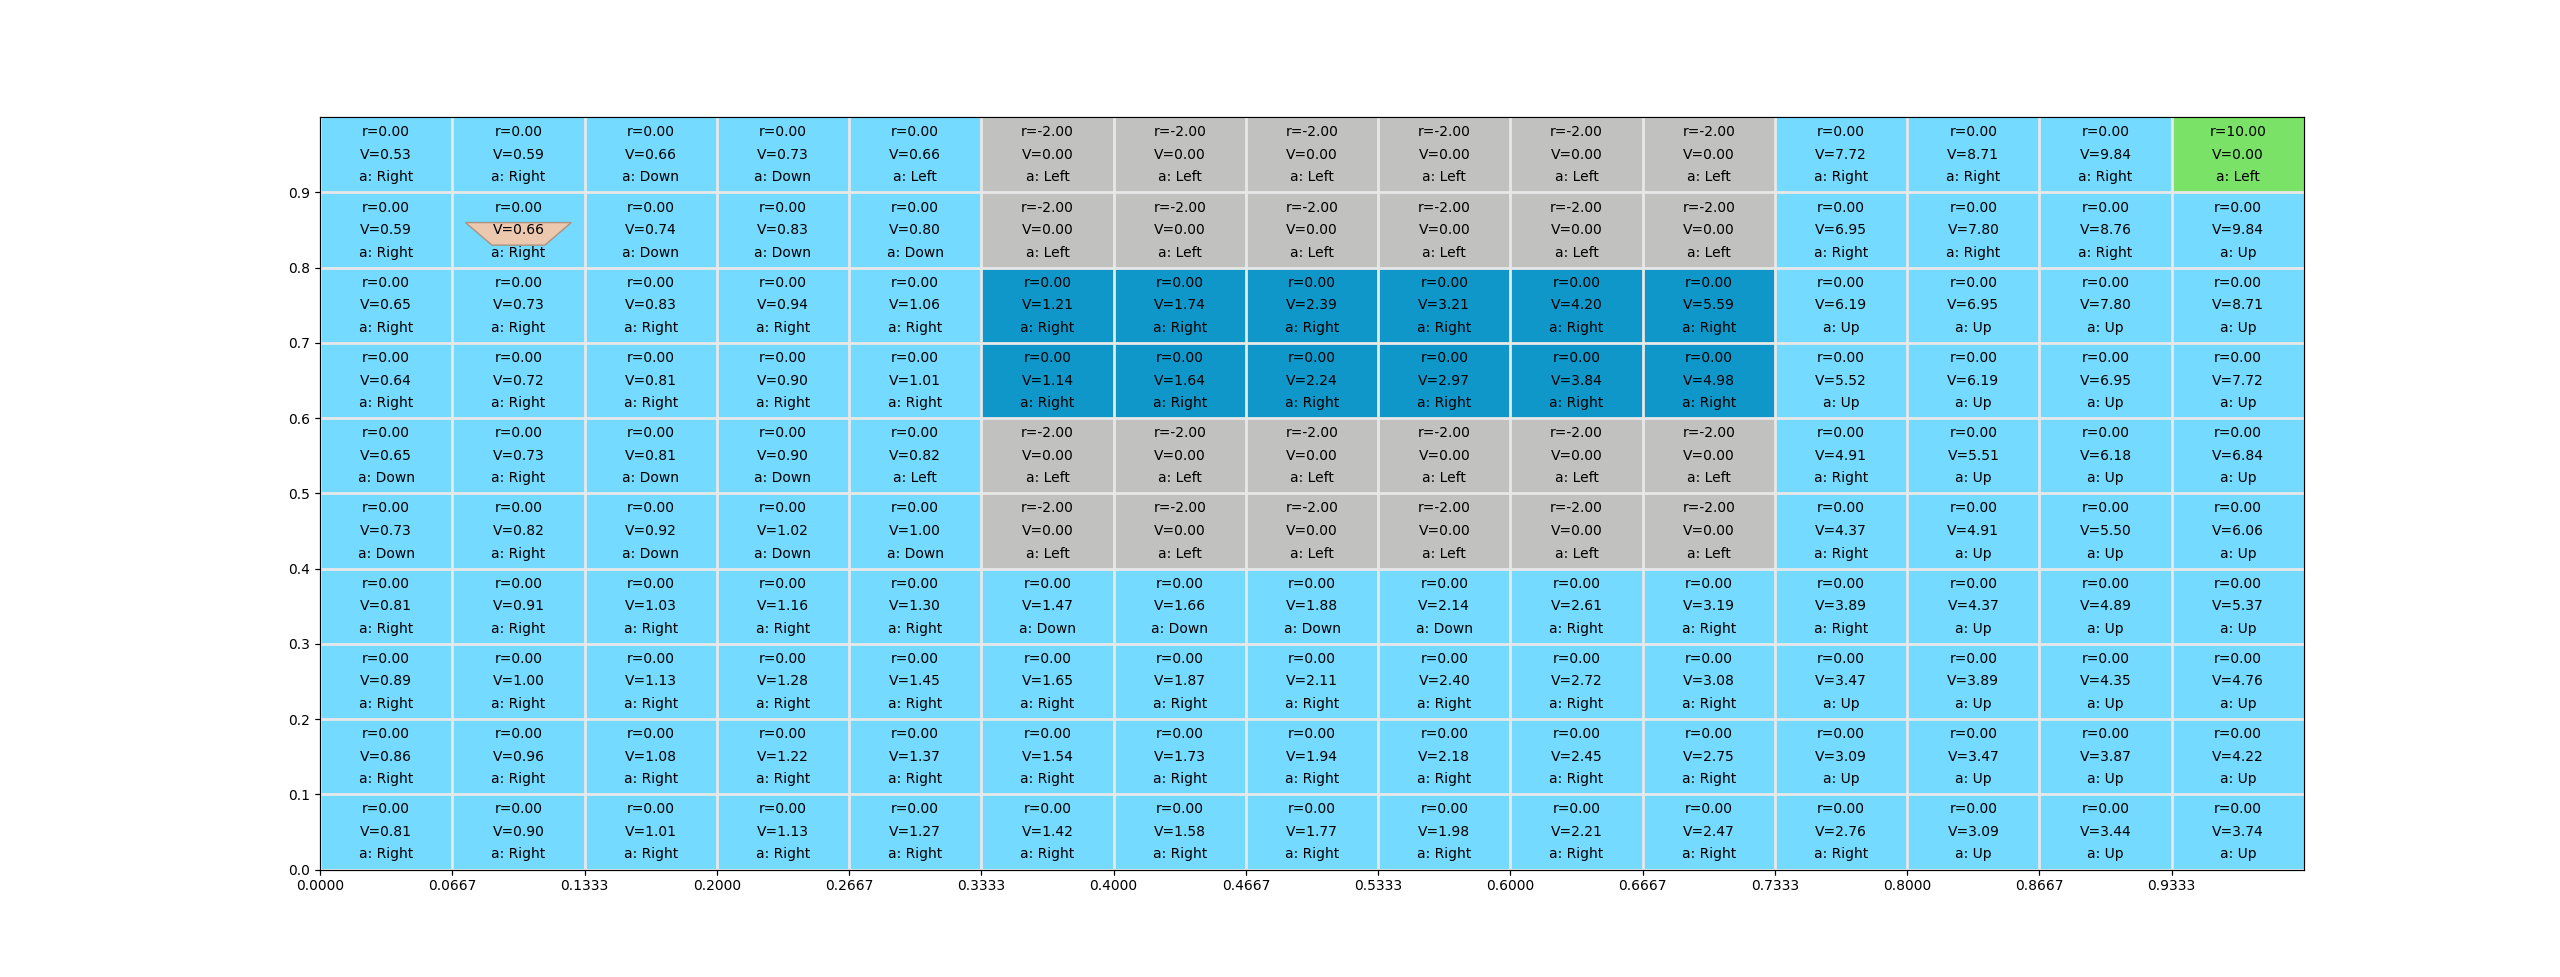
\includegraphics[scale=0.28]{exercise-2/report/img/final-board.png}
    \caption{Board with value function for each state, after iteration 100}
    \label{fig:my_label}
\end{figure}

\subsection{Question 2: What is the state value of the harbour and rock states? Why?}

The state-value function both for the rocks and for the harbour have the value of zero, this happens because those states are final states, so the episode finish if the agent reach them. And that also makes sense if we consider the value function as the expected reward when starting in state $s$, because if that state when we are \textit{starting} is final, then we could not expect more value.

\subsection{Task 2: compute the optimal policy}

Running the same value iteration algorithm as before, the optimal policy could be computed, as the action which gives us the best expected reward, and we can plot it in the similar board as the previous sections:



\bibliographystyle{ieeetr}
\bibliography{template}  % Modify template with your bibliography name
\end{document}
